\documentclass[12pt]{article}

\usepackage[margin=1in]{geometry}
\usepackage{graphicx}
\usepackage{booktabs}
\usepackage{float}
\usepackage{amsmath}
\usepackage{hyperref}
\usepackage{xcolor}
\usepackage{listings}
\usepackage{caption}
\usepackage{subcaption}

\hypersetup{
    colorlinks=true,
    linkcolor=blue,
    urlcolor=blue,
    citecolor=blue
}

\lstset{
    basicstyle=\ttfamily\small,
    breaklines=true,
    frame=single,
    numbers=left,
    numberstyle=\tiny,
    keywordstyle=\color{blue},
    commentstyle=\color{gray},
    showstringspaces=false
}

\title{CPU Scheduling Simulator\\
Performance Analysis and Algorithm Comparison}

\author{Ryan Kurz\\
CS 3502: Operating Systems\\
Kennesaw State University}

\date{July 23, 2026}

\begin{document}

\maketitle

\begin{abstract}
This project extends a Windows Forms CPU scheduling simulator by adding
Shortest Remaining Time First (SRTF) and Highest Response Ratio Next (HRRN).
The simulator calculates average waiting time, average turnaround time,
average response time, CPU utilization, and throughput. Six algorithms were
tested using small, medium, and large workloads to compare efficiency,
responsiveness, and fairness. The simulator was also extended with CSV
result export and interface documentation for the two new algorithms.
\end{abstract}

\tableofcontents
\newpage

\section{Introduction}

CPU scheduling determines which ready process receives access to the processor.
Different scheduling algorithms emphasize different goals, including low
waiting time, fast response, fairness, and protection from starvation.

The provided simulator already included First Come First Serve (FCFS),
Shortest Job First (SJF), Priority Scheduling, and Round Robin. This project
added Shortest Remaining Time First and Highest Response Ratio Next. The
interface was also extended to calculate performance metrics, display response
time, and export results to CSV files.

\section{Simulator Implementation}

\subsection{Starter Application}

The project uses C\# and Windows Forms. Process information is entered through
a table containing a process ID, burst time, priority, and arrival time. Each
algorithm produces a result containing the start time, finish time, waiting
time, turnaround time, and response time.

The original interface was kept and extended rather than replaced. Two new
algorithm buttons were added to the existing flow-layout panel. The Welcome
and About pages were updated to list all six algorithms, and the Results page
was expanded to display the required performance metrics.

\begin{figure}[H]
    \centering
    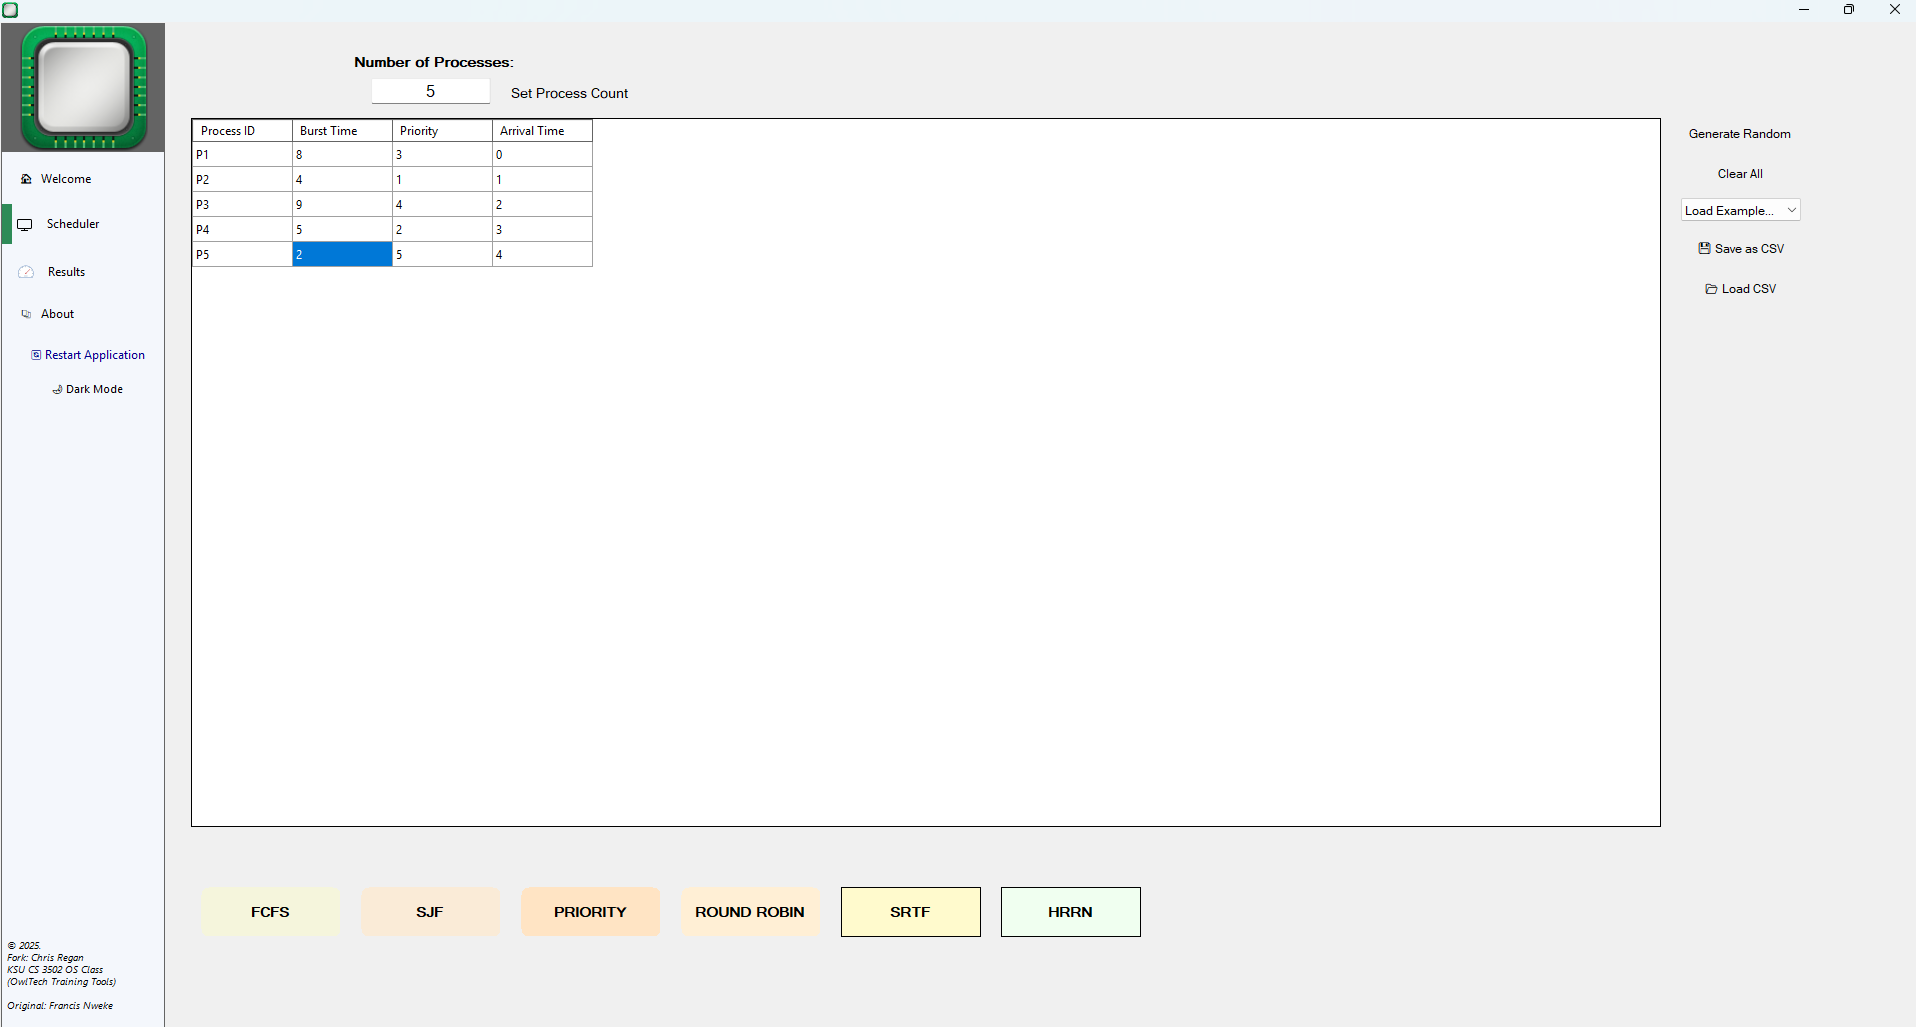
\includegraphics[width=\textwidth]{images/scheduler_all_algorithms.png}
    \caption{Scheduler page showing all six available algorithms.}
\end{figure}

\subsection{Shortest Remaining Time First}

Shortest Remaining Time First is the preemptive version of Shortest Job First.
At each unit of simulated time, the scheduler selects the available process
with the smallest remaining burst time. A newly arriving shorter process can
preempt the currently running process.

SRTF can reduce average waiting and turnaround time, especially when short
processes arrive after longer processes. Its main disadvantage is that long
processes may experience starvation if short processes continue to arrive.

The main implementation steps were:

\begin{enumerate}
    \item Store the remaining burst time for every process.
    \item At each time unit, collect all arrived processes that are not finished.
    \item Select the process with the smallest remaining time.
    \item Record its first start time if it has not run before.
    \item Execute it for one time unit.
    \item When it finishes, calculate finish, turnaround, and waiting times.
\end{enumerate}

\begin{lstlisting}[language=C,caption={Core SRTF selection logic}]
var availableProcesses = processes
    .Where(p => p.ArrivalTime <= currentTime &&
                remainingTimes[p.ProcessID] > 0)
    .OrderBy(p => remainingTimes[p.ProcessID])
    .ThenBy(p => p.ArrivalTime)
    .ThenBy(p => p.ProcessID)
    .ToList();

var currentProcess = availableProcesses.First();
remainingTimes[currentProcess.ProcessID]--;
currentTime++;
\end{lstlisting}

\begin{figure}[H]
    \centering
    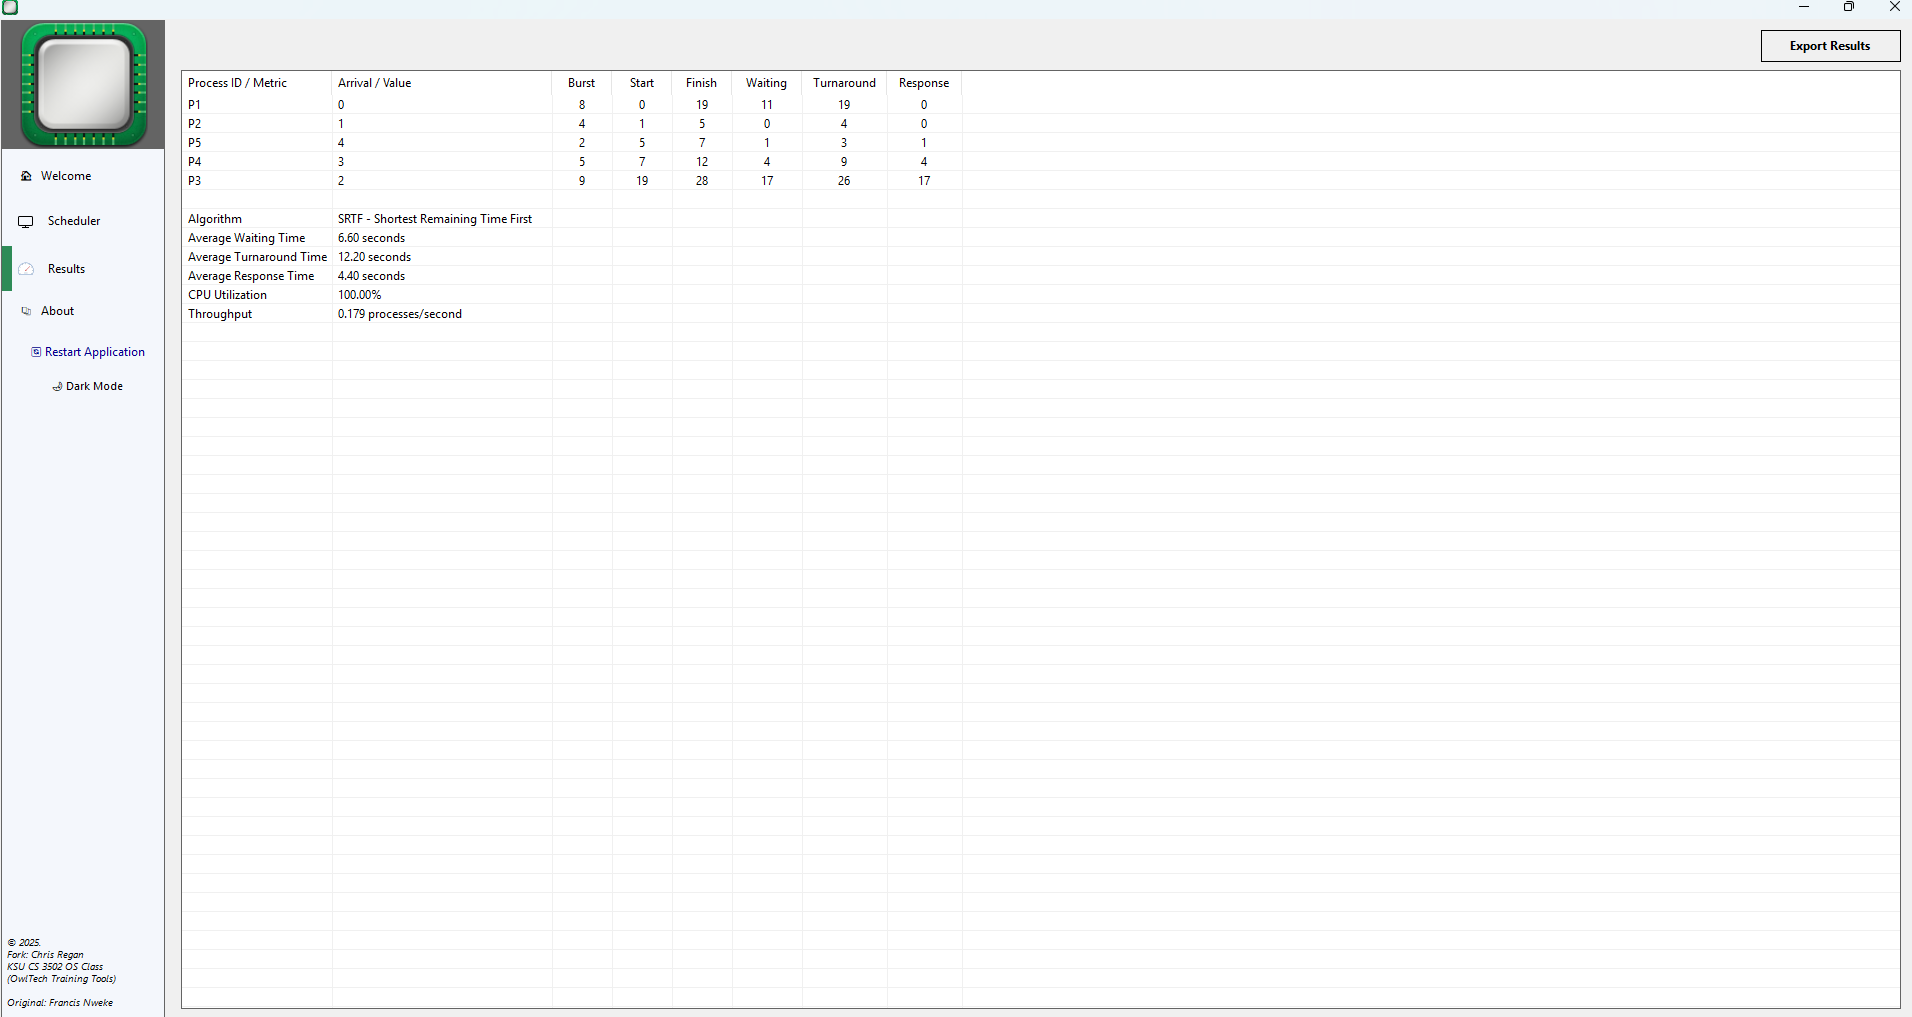
\includegraphics[width=\textwidth]{images/srtf_results.png}
    \caption{SRTF results for the small workload.}
\end{figure}

\subsection{Highest Response Ratio Next}

Highest Response Ratio Next is a non-preemptive scheduling algorithm. It selects
the available process with the highest response ratio:

\begin{equation}
R = \frac{W + B}{B}
\end{equation}

where \(W\) is waiting time and \(B\) is burst time.

This formula favors short jobs while gradually increasing the priority of
processes that have waited for a long time. HRRN therefore provides better
starvation protection than basic SJF.

The main implementation steps were:

\begin{enumerate}
    \item Collect all processes that have arrived by the current time.
    \item Calculate the response ratio for each available process.
    \item Select the process with the highest ratio.
    \item Run the selected process to completion.
    \item Calculate its waiting and turnaround times.
\end{enumerate}

\begin{lstlisting}[language=C,caption={Core HRRN selection logic}]
var nextProcess = availableProcesses
    .OrderByDescending(p =>
        ((double)(currentTime - p.ArrivalTime) + p.BurstTime)
        / p.BurstTime)
    .ThenBy(p => p.ArrivalTime)
    .ThenBy(p => p.ProcessID)
    .First();
\end{lstlisting}

\begin{figure}[H]
    \centering
    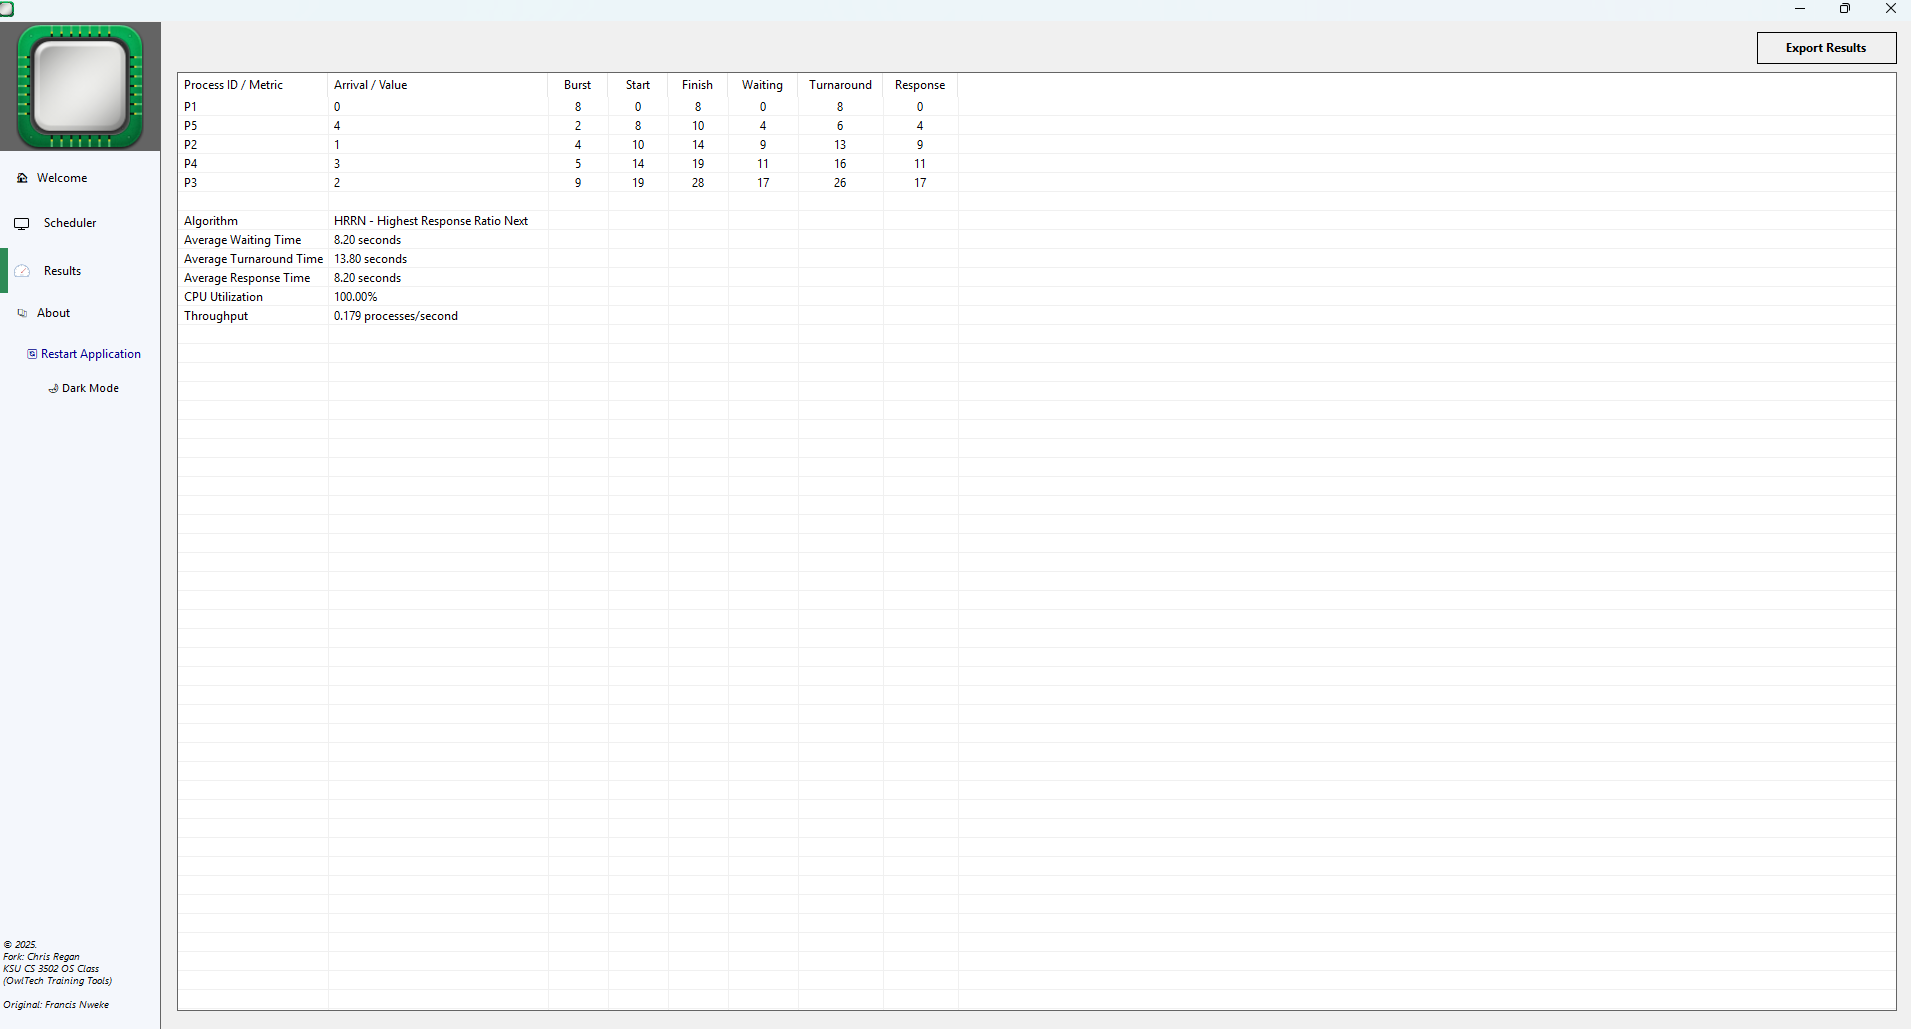
\includegraphics[width=\textwidth]{images/hrrn_results.png}
    \caption{HRRN results for the small workload.}
\end{figure}

\subsection{Performance Metrics and CSV Export}

The Results page was expanded to show one row per process and a separate set of
summary rows. The displayed metrics include average waiting time, average
turnaround time, average response time, CPU utilization, and throughput.

An Export Results button was also added. It writes the current process rows,
algorithm name, and metric rows to a CSV file. This made it possible to collect
results consistently for all workloads and algorithms.

\begin{figure}[H]
    \centering
    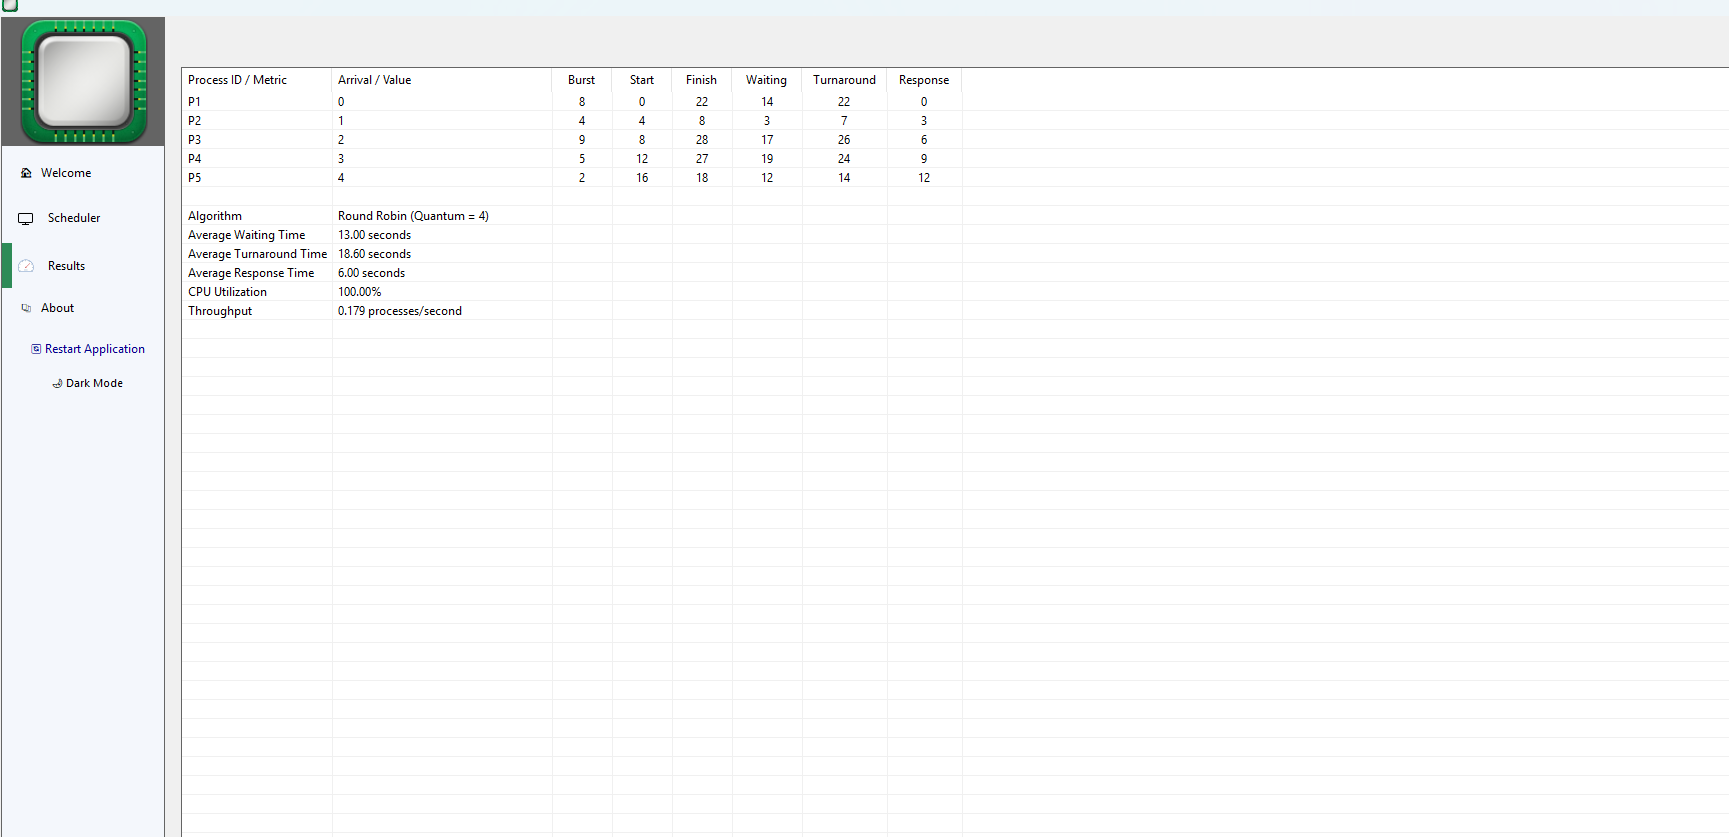
\includegraphics[width=\textwidth]{images/round_robin_results.png}
    \caption{Round Robin results with the Export Results button visible.}
\end{figure}

\section{Performance Metrics}

The following metrics were calculated for every algorithm.

\subsection{Average Waiting Time}

\begin{equation}
AWT = \frac{\sum_{i=1}^{n} W_i}{n}
\end{equation}

\subsection{Average Turnaround Time}

\begin{equation}
ATT = \frac{\sum_{i=1}^{n} T_i}{n}
\end{equation}

\subsection{Average Response Time}

\begin{equation}
ART = \frac{\sum_{i=1}^{n} (S_i - A_i)}{n}
\end{equation}

where \(S_i\) is the first start time and \(A_i\) is the arrival time.

\subsection{CPU Utilization}

\begin{equation}
CPU\ Utilization =
\frac{\text{Total Burst Time}}{\text{Total Elapsed Time}} \times 100
\end{equation}

\subsection{Throughput}

\begin{equation}
Throughput =
\frac{\text{Number of Completed Processes}}{\text{Total Elapsed Time}}
\end{equation}

\section{Testing Method}

Three main workload sizes were tested:

\begin{itemize}
    \item Small workload: 5 processes
    \item Medium workload: 20 processes
    \item Large workload: 100 processes
\end{itemize}

All six algorithms were tested using the same process data for each workload.
Round Robin used a time quantum of 4. The small workload was manually defined,
the medium workload used mixed burst and arrival times, and the large workload
used heavier burst times. An additional idle-gap workload was used to verify
that CPU utilization correctly decreases when no process is ready.

\section{Results}

\subsection{Small Workload}

\begin{table}[H]
\centering
\caption{Small workload performance}
\begin{tabular}{lrrr}
\toprule
Algorithm & Avg. Wait & Avg. Turnaround & Avg. Response \\
\midrule
FCFS & 11.40 & 17.00 & 11.40 \\
SJF & 8.20 & 13.80 & 8.20 \\
Priority & 10.20 & 15.80 & 10.20 \\
Round Robin & 13.00 & 18.60 & 6.00 \\
SRTF & 6.60 & 12.20 & 4.40 \\
HRRN & 8.20 & 13.80 & 8.20 \\
\bottomrule
\end{tabular}
\end{table}

For the small workload, SRTF produced the lowest average waiting time,
turnaround time, and response time.

\subsection{Medium Workload}

\begin{table}[H]
\centering
\caption{Medium workload performance}
\begin{tabular}{lrrr}
\toprule
Algorithm & Avg. Wait & Avg. Turnaround & Avg. Response \\
\midrule
FCFS & 104.15 & 115.20 & 104.15 \\
SJF & 74.65 & 85.70 & 74.65 \\
Priority & 103.80 & 114.85 & 103.80 \\
Round Robin & 161.35 & 172.40 & 35.00 \\
SRTF & 73.15 & 84.20 & 68.85 \\
HRRN & 78.90 & 89.95 & 78.90 \\
\bottomrule
\end{tabular}
\end{table}

For the medium workload, SRTF again produced the lowest waiting and turnaround
times. Round Robin produced the lowest response time but substantially higher
waiting and turnaround times.

\subsection{Large Workload}

\begin{table}[H]
\centering
\caption{Large workload performance}
\begin{tabular}{lrrr}
\toprule
Algorithm & Avg. Wait & Avg. Turnaround & Avg. Response \\
\midrule
FCFS & 1002.27 & 1022.64 & 1002.27 \\
SJF & 831.02 & 851.39 & 831.02 \\
Priority & 1008.06 & 1028.43 & 1008.06 \\
Round Robin & 1771.49 & 1791.86 & 195.58 \\
SRTF & 831.02 & 851.39 & 831.02 \\
HRRN & 839.56 & 859.93 & 839.56 \\
\bottomrule
\end{tabular}
\end{table}

For the large workload, SJF and SRTF tied for the lowest waiting and turnaround
times. Round Robin again produced the lowest response time but the highest
waiting and turnaround times.

\subsection{Performance Trends}

\begin{figure}[H]
    \centering
    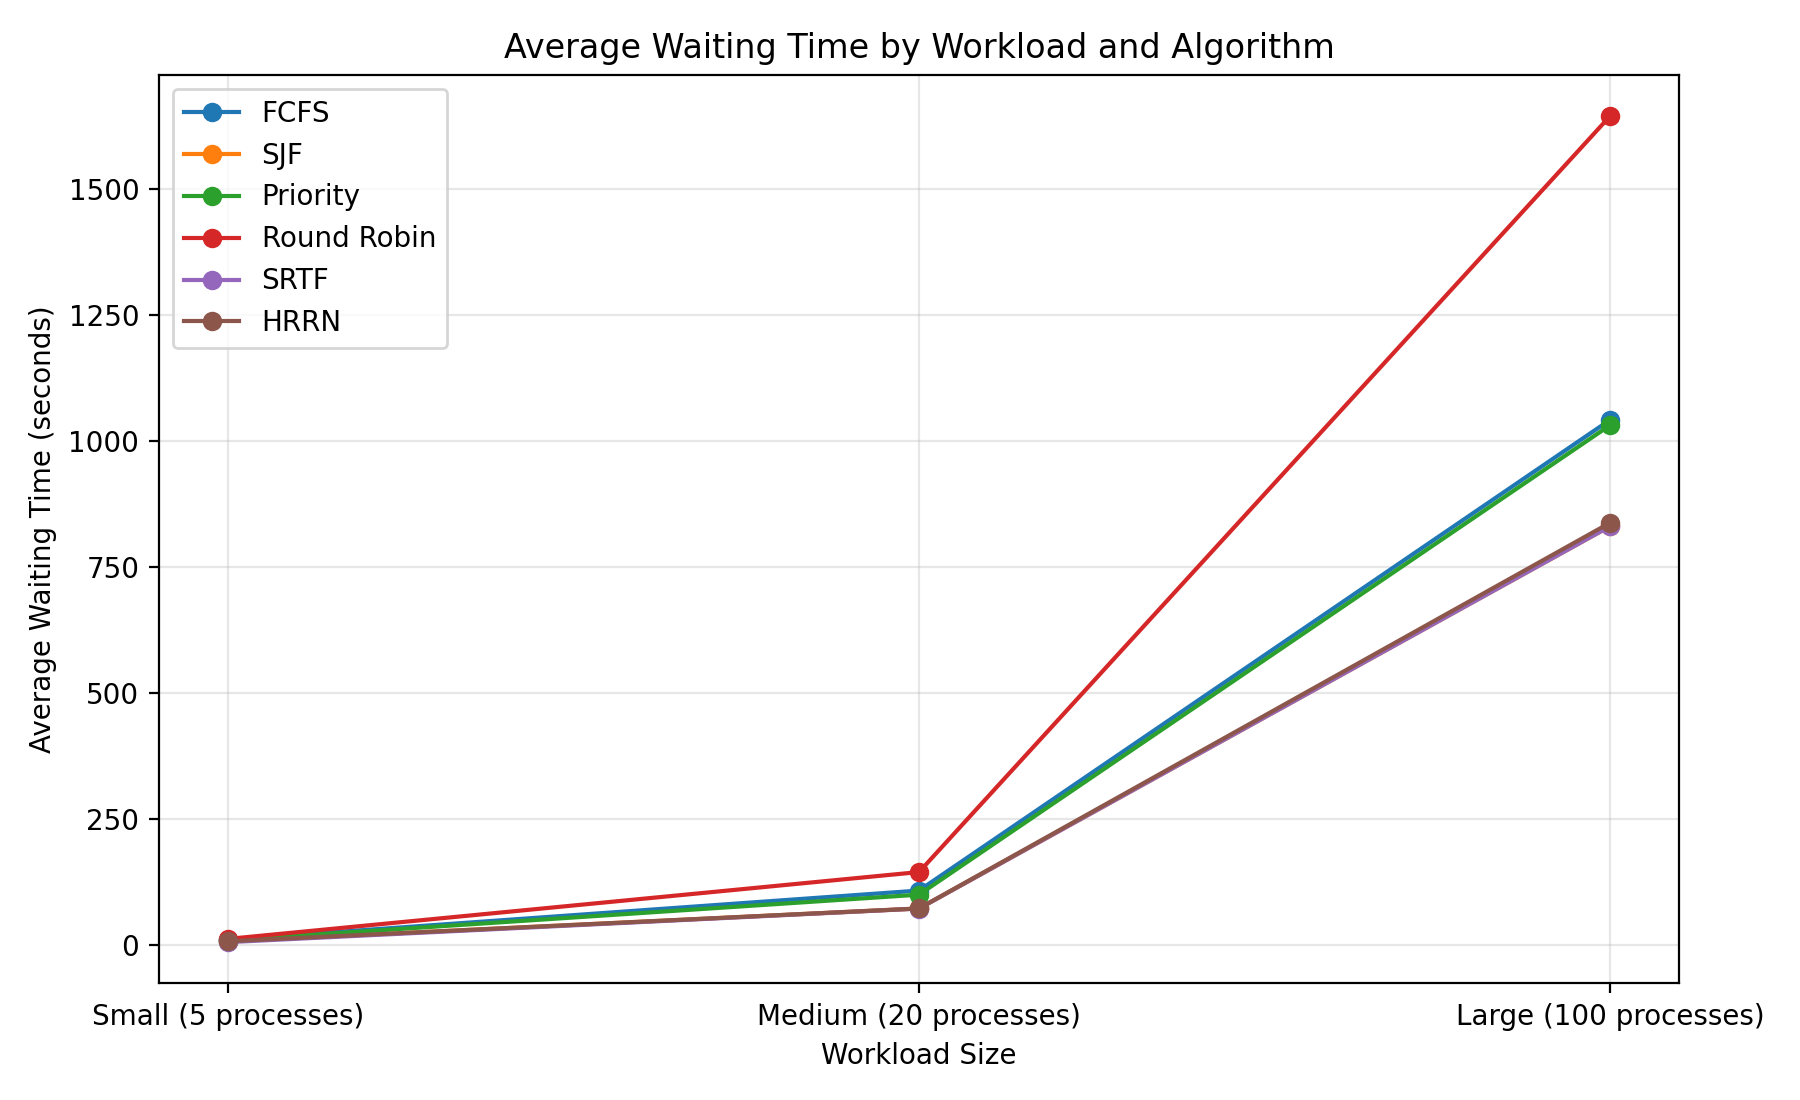
\includegraphics[width=0.9\textwidth]{images/average_waiting_time.png}
    \caption{Average waiting time by workload and algorithm.}
\end{figure}

\begin{figure}[H]
    \centering
    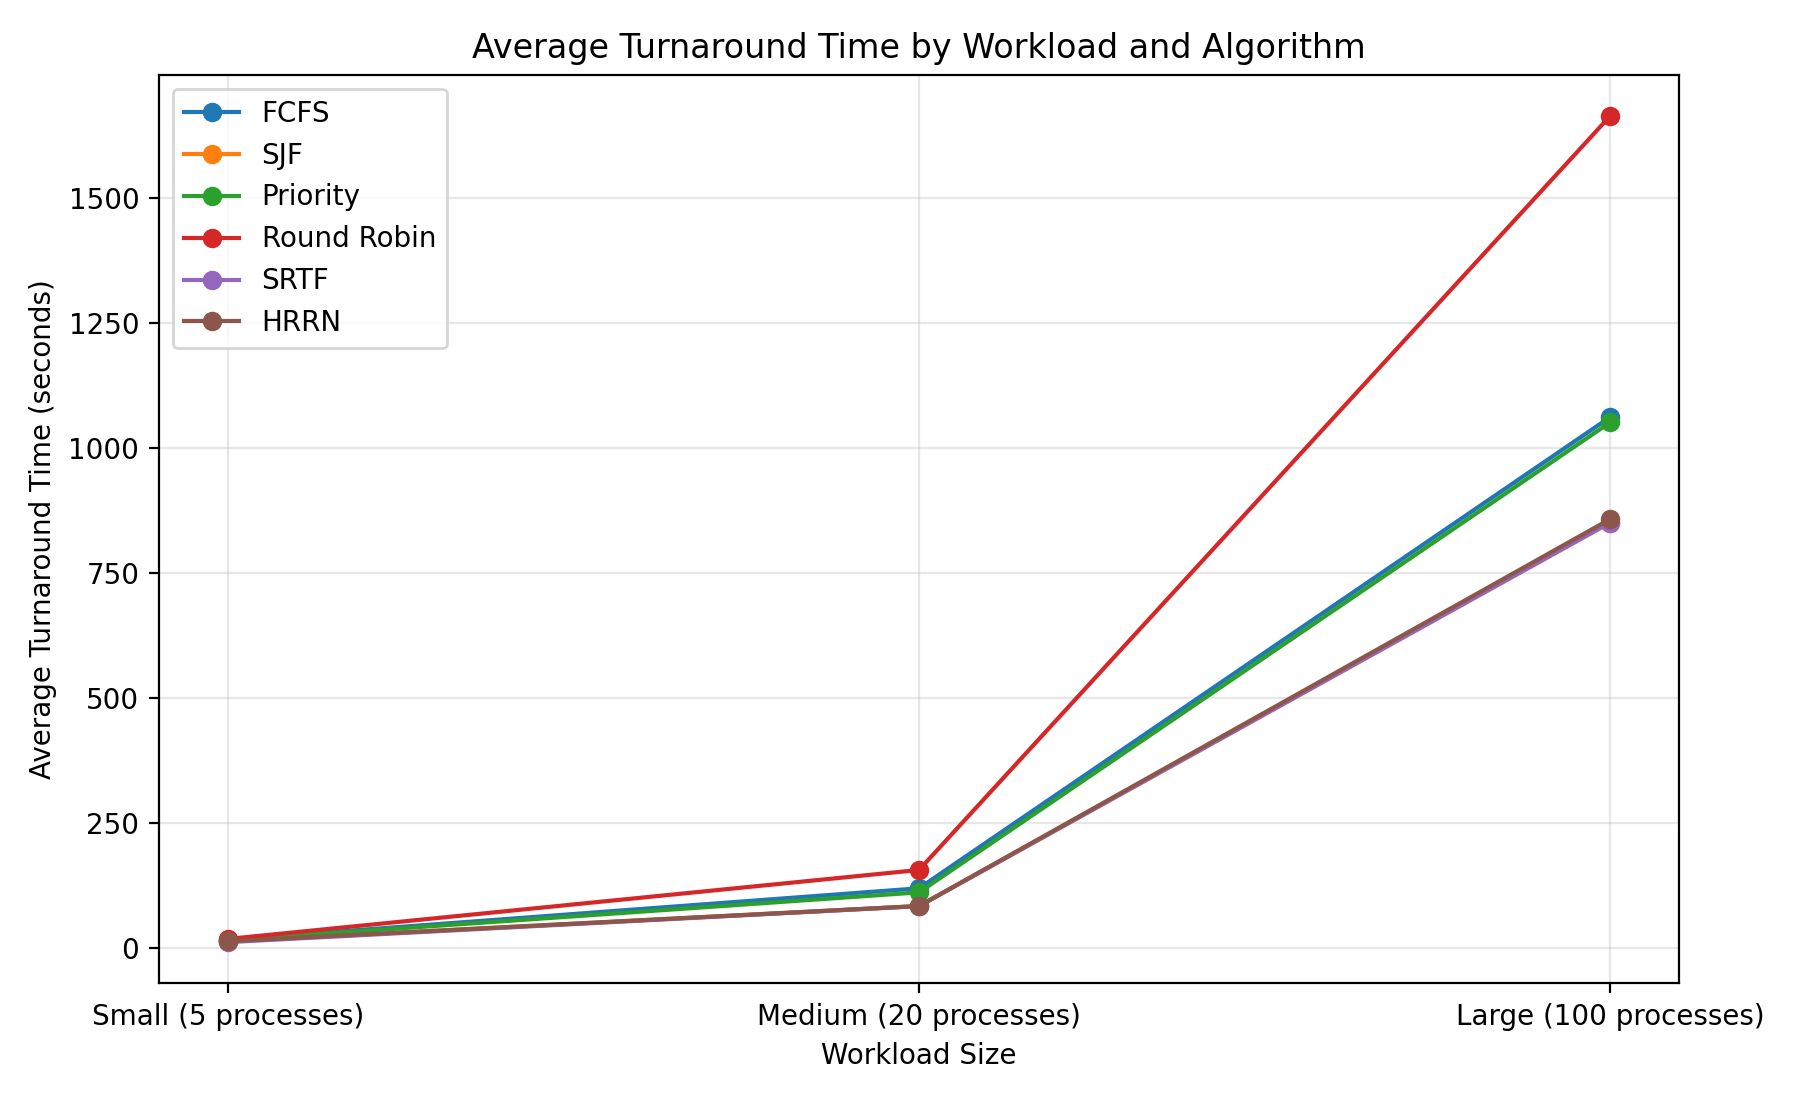
\includegraphics[width=0.9\textwidth]{images/average_turnaround_time.png}
    \caption{Average turnaround time by workload and algorithm.}
\end{figure}

\begin{figure}[H]
    \centering
    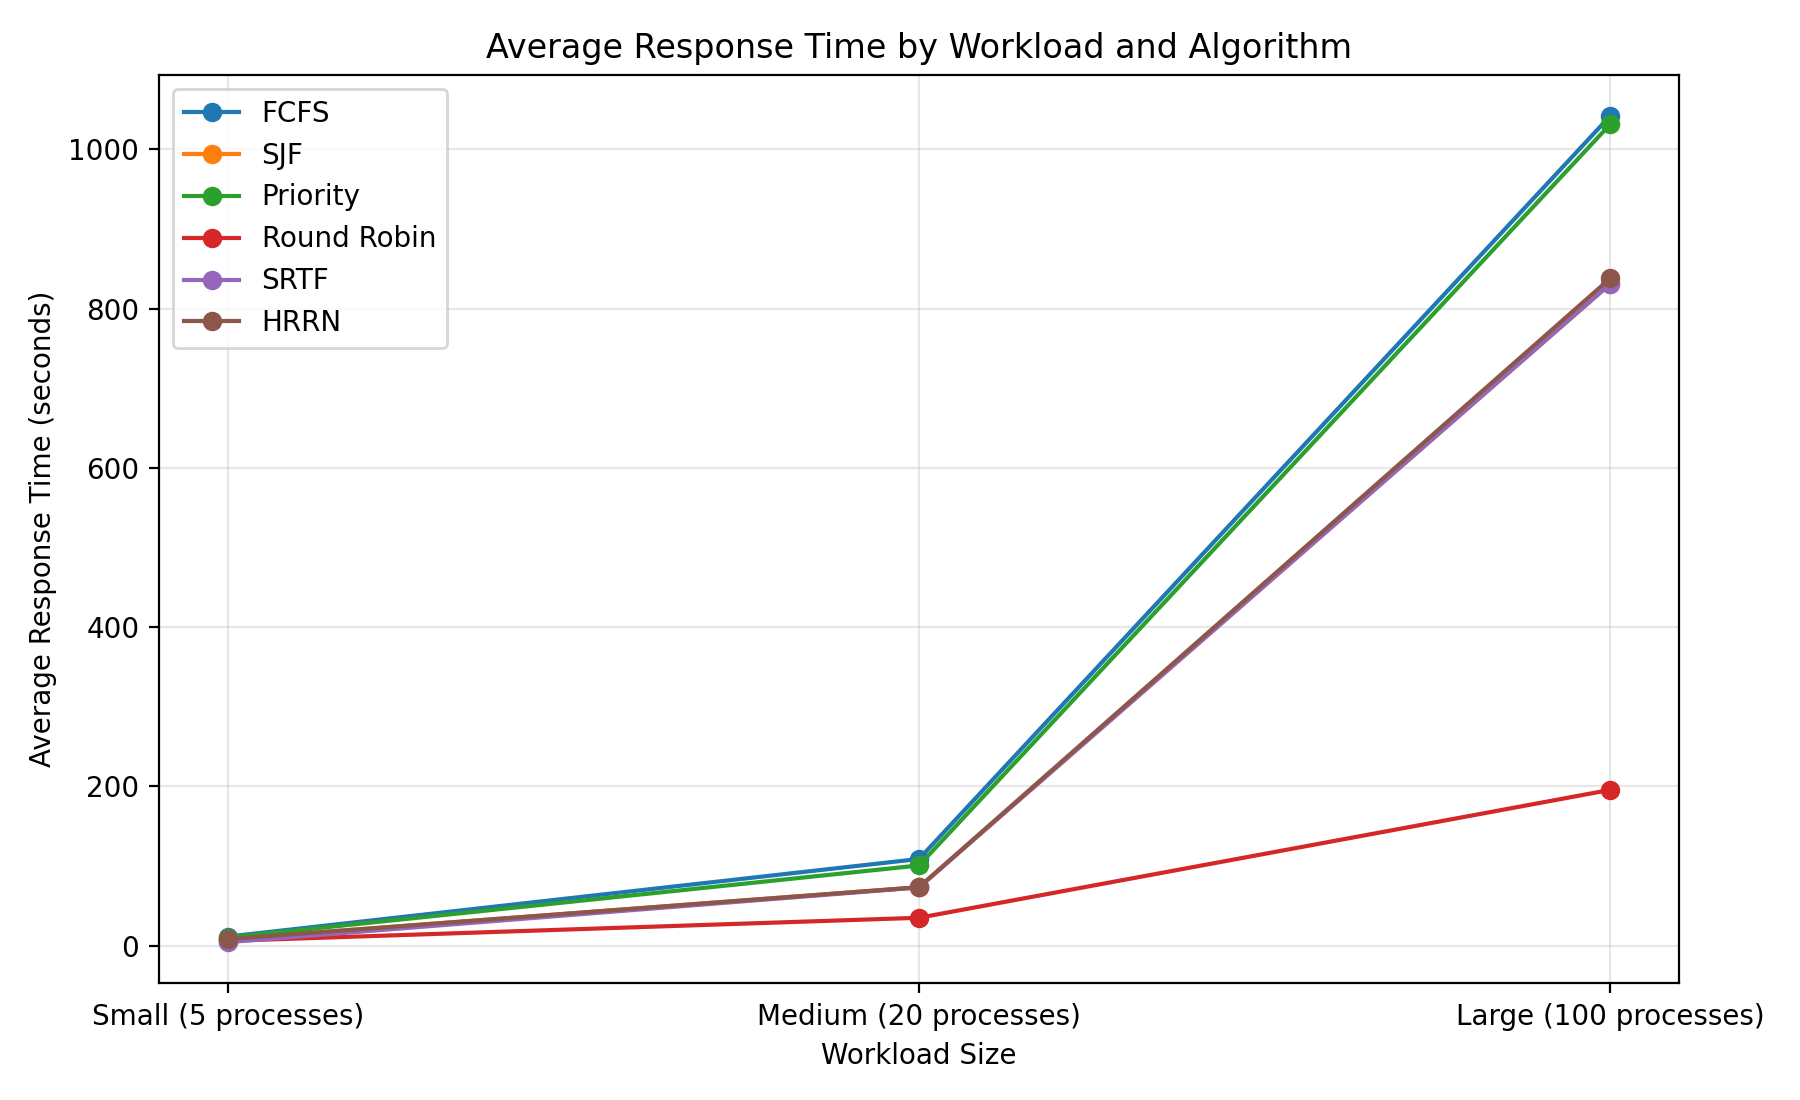
\includegraphics[width=0.9\textwidth]{images/average_response_time.png}
    \caption{Average response time by workload and algorithm.}
\end{figure}

The graphs show that waiting and turnaround times rise significantly as the
number of processes increases. SJF, SRTF, and HRRN scale better than FCFS,
Priority, and Round Robin for waiting and turnaround time. Round Robin scales
poorly for completion-related metrics but remains strong for initial response.

\section{Analysis and Trade-Offs}

SRTF produced the best or tied-best average waiting and turnaround times across
the tested workloads. This occurred because it always favored the process with
the least remaining work. However, this strategy can delay long processes when
short jobs continue to arrive.

SJF performed similarly to SRTF on the large workload because the generated
arrival pattern did not create enough useful preemption opportunities to give
SRTF an advantage. SJF is simpler because it is non-preemptive, but it can also
starve long processes.

HRRN stayed close to SJF while providing better starvation protection. Its
response-ratio formula increases a process's chance of selection as its waiting
time grows. This makes it a reasonable compromise between efficiency and
fairness.

Round Robin produced the best response time for the medium and large workloads.
Every process received an early time slice, which improves responsiveness.
However, repeated queue cycling increased average waiting and turnaround times.
In a real operating system, context-switch overhead would make this trade-off
even more significant.

FCFS was simple and predictable but suffered from the convoy effect when long
processes appeared before short ones. Priority Scheduling depended heavily on
the assigned priorities and can starve low-priority processes without aging.

CPU utilization and throughput were the same for algorithms within each main
workload because they processed the same total burst time without idle periods.
The meaningful differences were therefore waiting, turnaround, and response
times.

\section{Idle CPU Validation}

An additional test used three processes with arrival times of 0, 10, and 12.
The CPU was idle between time 3 and time 10. The simulator reported CPU
utilization of 56.25 percent, matching the manual calculation:

\begin{equation}
\frac{3 + 2 + 4}{16} \times 100 = 56.25\%
\end{equation}

This confirmed that idle time was included correctly in the utilization
calculation.

\begin{figure}[H]
    \centering
    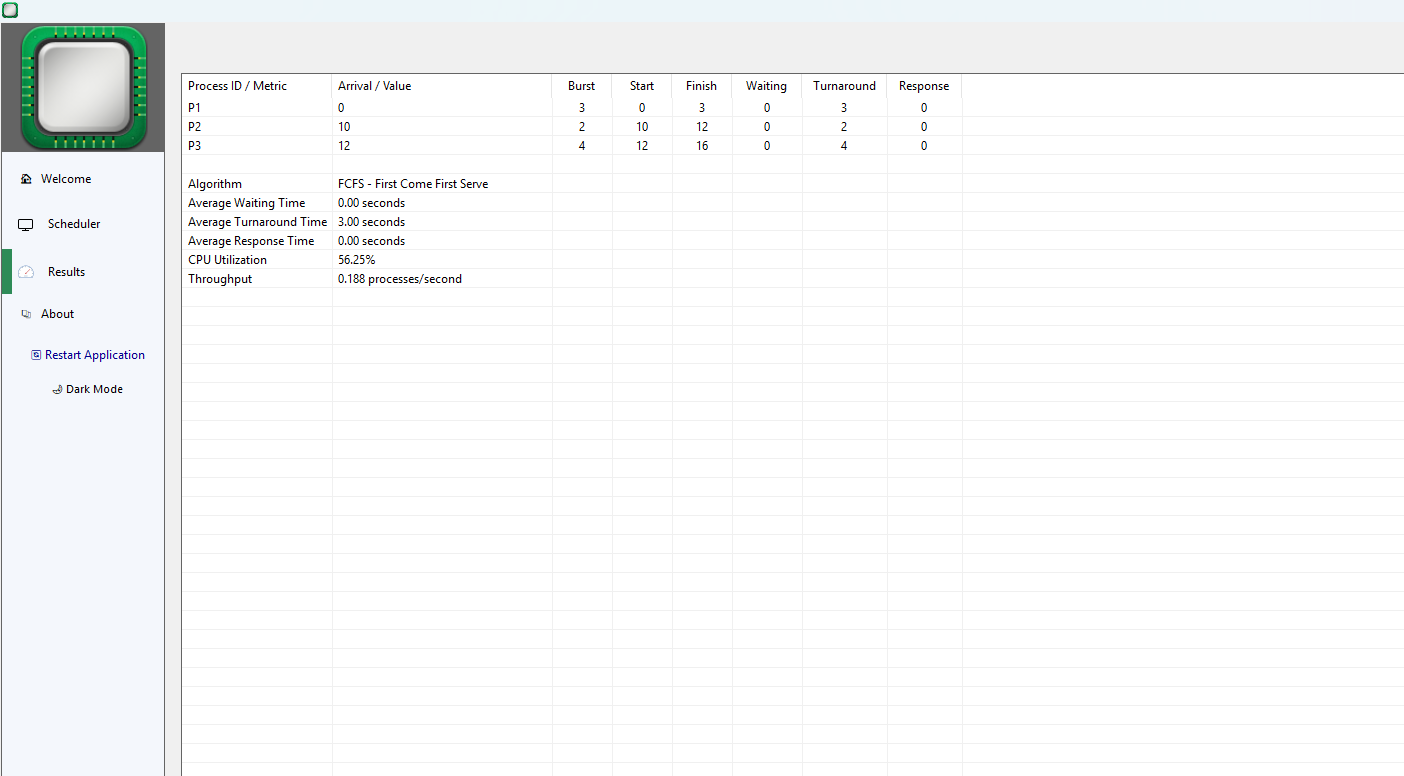
\includegraphics[width=\textwidth]{images/idle_gap_test.png}
    \caption{Idle-gap validation showing 56.25 percent CPU utilization.}
\end{figure}

\section{Recommendation}

For workloads where minimizing waiting and turnaround time is the main goal,
OwlTech should use SRTF. It performed best or near best across the tested
workloads.

For interactive systems where fast initial response and fairness are more
important, Round Robin is preferable. However, its time quantum must be chosen
carefully because a small quantum increases queue cycling and context switching.

HRRN is recommended when starvation prevention is important but the system
still needs performance similar to SJF. It provides a strong balance between
efficiency and fairness without requiring preemption.

\section{Future Improvements}

Possible future improvements include:

\begin{itemize}
    \item Adding a Gantt chart timeline
    \item Supporting Multilevel Feedback Queue scheduling
    \item Automatically running every algorithm on one workload
    \item Exporting a combined comparison CSV
    \item Measuring actual simulator execution time
    \item Adding context-switch overhead
    \item Adding priority aging
    \item Letting the user compare algorithms side by side in the interface
\end{itemize}

\section{Conclusion}

The project successfully added SRTF and HRRN to the provided CPU scheduling
simulator. It also added response time, CPU utilization, throughput, CSV export,
updated interface documentation, and expanded result display functionality.

Testing showed that no single algorithm is ideal for every workload. SRTF
provided strong waiting and turnaround performance, Round Robin provided fast
response, and HRRN offered a useful balance between efficiency and fairness.
The final recommendation depends on whether the target system values completion
time, responsiveness, or starvation prevention most strongly.

\begin{thebibliography}{9}

\bibitem{project}
CS 3502 Project 2: CPU Scheduling Simulator, Kennesaw State University,
Department of Computer Science, 2026.

\bibitem{starter}
CPU-Simulator using Windows Forms, starter repository maintained by Chris
Regan, original creator Francis.

\bibitem{cpu}
J. Bell, ``CPU Scheduling,'' Operating Systems Course Notes,
University of Illinois Chicago.

\end{thebibliography}

\end{document}
